% Source-faithful schematic draft: src-6914e1c400640e0c3ef3785cb187876891213e18557a04ba0e97c2f4dae5a999
% Source SHA-256 32093147448a616af26055d81831b7028e661e5138d8546f803a6c6a1a42bc43; PDF p.1, Q19.
% Diagram topology only; no measurements, angle, or additional incidence claims beyond visible projections.
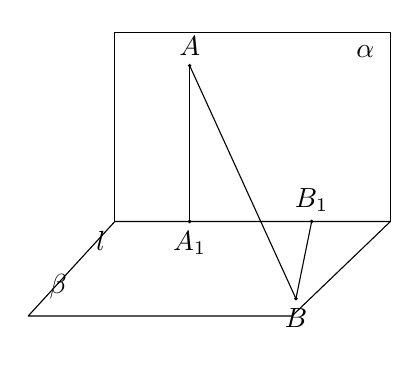
\begin{tikzpicture}[line join=round, line cap=round]
  \draw (0,0) -- (3.5,0) -- (3.5,2.4) -- (0,2.4) -- cycle;
  \node at (3.18,2.16) {$\alpha$};
  \draw (0,0) -- (3.5,0) -- (2.25,-1.2) -- (-1.1,-1.2) -- cycle;
  \node at (-0.72,-0.83) {$\beta$};
  \node[below left] at (0,0) {$l$};
  \coordinate (A) at (0.95,1.98);
  \coordinate (Aone) at (0.95,0);
  \coordinate (B) at (2.30,-0.98);
  \coordinate (Bone) at (2.50,0);
  \draw (A)--(B);
  \draw (A)--(Aone);
  \draw (B)--(Bone);
  \fill (A) circle (0.7pt) node[above] {$A$};
  \fill (B) circle (0.7pt) node[below] {$B$};
  \fill (Aone) circle (0.7pt) node[below] {$A_1$};
  \fill (Bone) circle (0.7pt) node[above] {$B_1$};
\end{tikzpicture}
